\documentclass[twoside]{book}

% Packages required by doxygen
\usepackage{fixltx2e}
\usepackage{calc}
\usepackage{doxygen}
\usepackage[export]{adjustbox} % also loads graphicx
\usepackage{graphicx}
\usepackage[utf8]{inputenc}
\usepackage{makeidx}
\usepackage{multicol}
\usepackage{multirow}
\PassOptionsToPackage{warn}{textcomp}
\usepackage{textcomp}
\usepackage[nointegrals]{wasysym}
\usepackage[table]{xcolor}

% Font selection
\usepackage[T1]{fontenc}
\usepackage[scaled=.90]{helvet}
\usepackage{courier}
\usepackage{amssymb}
\usepackage{sectsty}
\renewcommand{\familydefault}{\sfdefault}
\allsectionsfont{%
  \fontseries{bc}\selectfont%
  \color{darkgray}%
}
\renewcommand{\DoxyLabelFont}{%
  \fontseries{bc}\selectfont%
  \color{darkgray}%
}
\newcommand{\+}{\discretionary{\mbox{\scriptsize$\hookleftarrow$}}{}{}}

% Page & text layout
\usepackage{geometry}
\geometry{%
  a4paper,%
  top=2.5cm,%
  bottom=2.5cm,%
  left=2.5cm,%
  right=2.5cm%
}
\tolerance=750
\hfuzz=15pt
\hbadness=750
\setlength{\emergencystretch}{15pt}
\setlength{\parindent}{0cm}
\setlength{\parskip}{3ex plus 2ex minus 2ex}
\makeatletter
\renewcommand{\paragraph}{%
  \@startsection{paragraph}{4}{0ex}{-1.0ex}{1.0ex}{%
    \normalfont\normalsize\bfseries\SS@parafont%
  }%
}
\renewcommand{\subparagraph}{%
  \@startsection{subparagraph}{5}{0ex}{-1.0ex}{1.0ex}{%
    \normalfont\normalsize\bfseries\SS@subparafont%
  }%
}
\makeatother

% Headers & footers
\usepackage{fancyhdr}
\pagestyle{fancyplain}
\fancyhead[LE]{\fancyplain{}{\bfseries\thepage}}
\fancyhead[CE]{\fancyplain{}{}}
\fancyhead[RE]{\fancyplain{}{\bfseries\leftmark}}
\fancyhead[LO]{\fancyplain{}{\bfseries\rightmark}}
\fancyhead[CO]{\fancyplain{}{}}
\fancyhead[RO]{\fancyplain{}{\bfseries\thepage}}
\fancyfoot[LE]{\fancyplain{}{}}
\fancyfoot[CE]{\fancyplain{}{}}
\fancyfoot[RE]{\fancyplain{}{\bfseries\scriptsize Generated by Doxygen }}
\fancyfoot[LO]{\fancyplain{}{\bfseries\scriptsize Generated by Doxygen }}
\fancyfoot[CO]{\fancyplain{}{}}
\fancyfoot[RO]{\fancyplain{}{}}
\renewcommand{\footrulewidth}{0.4pt}
\renewcommand{\chaptermark}[1]{%
  \markboth{#1}{}%
}
\renewcommand{\sectionmark}[1]{%
  \markright{\thesection\ #1}%
}

% Indices & bibliography
\usepackage{natbib}
\usepackage[titles]{tocloft}
\setcounter{tocdepth}{3}
\setcounter{secnumdepth}{5}
\makeindex

% Hyperlinks (required, but should be loaded last)
\usepackage{ifpdf}
\ifpdf
  \usepackage[pdftex,pagebackref=true]{hyperref}
\else
  \usepackage[ps2pdf,pagebackref=true]{hyperref}
\fi
\hypersetup{%
  colorlinks=true,%
  linkcolor=blue,%
  citecolor=blue,%
  unicode%
}

% Custom commands
\newcommand{\clearemptydoublepage}{%
  \newpage{\pagestyle{empty}\cleardoublepage}%
}

\usepackage{caption}
\captionsetup{labelsep=space,justification=centering,font={bf},singlelinecheck=off,skip=4pt,position=top}

%===== C O N T E N T S =====

\begin{document}

% Titlepage & ToC
\hypersetup{pageanchor=false,
             bookmarksnumbered=true,
             pdfencoding=unicode
            }
\pagenumbering{roman}
\begin{titlepage}
\vspace*{7cm}
\begin{center}%
{\Large My Project }\\
\vspace*{1cm}
{\large Generated by Doxygen 1.8.11}\\
\end{center}
\end{titlepage}
\clearemptydoublepage
\tableofcontents
\clearemptydoublepage
\pagenumbering{arabic}
\hypersetup{pageanchor=true}

%--- Begin generated contents ---
\chapter{File Index}
\section{File List}
Here is a list of all files with brief descriptions\+:\begin{DoxyCompactList}
\item\contentsline{section}{\hyperlink{Lab1_8c}{Lab1.\+c} }{\pageref{Lab1_8c}}{}
\end{DoxyCompactList}

\chapter{File Documentation}
\hypertarget{EuclidianAlg_8cpp}{}\section{Euclidian\+Alg.\+cpp File Reference}
\label{EuclidianAlg_8cpp}\index{Euclidian\+Alg.\+cpp@{Euclidian\+Alg.\+cpp}}
{\ttfamily \#include $<$iostream$>$}\\*
{\ttfamily \#include $<$utility$>$}\\*
Include dependency graph for Euclidian\+Alg.\+cpp\+:
\nopagebreak
\begin{figure}[H]
\begin{center}
\leavevmode
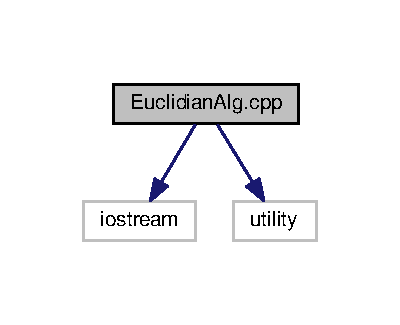
\includegraphics[width=192pt]{EuclidianAlg_8cpp__incl}
\end{center}
\end{figure}
\subsection*{Functions}
\begin{DoxyCompactItemize}
\item 
pair$<$ int, pair$<$ int, int $>$ $>$ \hyperlink{EuclidianAlg_8cpp_a8cf629c2377f5a483790e9ffb92a9001}{extended\+Euclid} (int a, int b)
\item 
int \hyperlink{EuclidianAlg_8cpp_a95942be30ba56c0c3d82cf4c89fbdcdb}{mod\+Inverse} (int a, int m)
\item 
int \hyperlink{EuclidianAlg_8cpp_ae66f6b31b5ad750f1fe042a706a4e3d4}{main} ()
\end{DoxyCompactItemize}


\subsection{Function Documentation}
\index{Euclidian\+Alg.\+cpp@{Euclidian\+Alg.\+cpp}!extended\+Euclid@{extended\+Euclid}}
\index{extended\+Euclid@{extended\+Euclid}!Euclidian\+Alg.\+cpp@{Euclidian\+Alg.\+cpp}}
\subsubsection[{\texorpdfstring{extended\+Euclid(int a, int b)}{extendedEuclid(int a, int b)}}]{\setlength{\rightskip}{0pt plus 5cm}pair$<$int, pair$<$int, int$>$ $>$ extended\+Euclid (
\begin{DoxyParamCaption}
\item[{int}]{a, }
\item[{int}]{b}
\end{DoxyParamCaption}
)}\hypertarget{EuclidianAlg_8cpp_a8cf629c2377f5a483790e9ffb92a9001}{}\label{EuclidianAlg_8cpp_a8cf629c2377f5a483790e9ffb92a9001}

\begin{DoxyCode}
12 \{
13     \textcolor{keywordtype}{int} x = 1, y = 0;
14     \textcolor{keywordtype}{int} xLast = 0, yLast = 1;
15     \textcolor{keywordtype}{int} q, r, m, n;
16     \textcolor{keywordflow}{while} (a != 0) 
17     \{
18         q = b / a;
19         r = b % a;
20         m = xLast - q * x;
21         n = yLast - q * y;
22         xLast = x; 
23         yLast = y;
24         x = m; 
25         y = n;
26         b = a; 
27         a = r;
28     \}
29     \textcolor{keywordflow}{return} make\_pair(b, make\_pair(xLast, yLast));
30 \}
\end{DoxyCode}
\index{Euclidian\+Alg.\+cpp@{Euclidian\+Alg.\+cpp}!main@{main}}
\index{main@{main}!Euclidian\+Alg.\+cpp@{Euclidian\+Alg.\+cpp}}
\subsubsection[{\texorpdfstring{main()}{main()}}]{\setlength{\rightskip}{0pt plus 5cm}int main (
\begin{DoxyParamCaption}
{}
\end{DoxyParamCaption}
)}\hypertarget{EuclidianAlg_8cpp_ae66f6b31b5ad750f1fe042a706a4e3d4}{}\label{EuclidianAlg_8cpp_ae66f6b31b5ad750f1fe042a706a4e3d4}

\begin{DoxyCode}
39 \{
40     \textcolor{keywordtype}{int} a, m;
41     cout<<\textcolor{stringliteral}{"Enter number to find modular multiplicative inverse: "};
42     cin>>a;
43     cout<<\textcolor{stringliteral}{"Enter Modular Value: "};
44     cin>>m;
45     cout<<\hyperlink{EuclidianAlg_8cpp_a95942be30ba56c0c3d82cf4c89fbdcdb}{modInverse}(a, m)<<endl;
46 \}
\end{DoxyCode}


Here is the call graph for this function\+:
\nopagebreak
\begin{figure}[H]
\begin{center}
\leavevmode
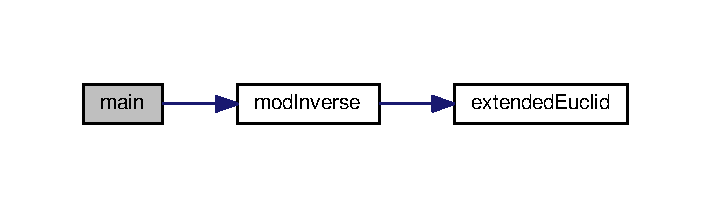
\includegraphics[width=341pt]{EuclidianAlg_8cpp_ae66f6b31b5ad750f1fe042a706a4e3d4_cgraph}
\end{center}
\end{figure}


\index{Euclidian\+Alg.\+cpp@{Euclidian\+Alg.\+cpp}!mod\+Inverse@{mod\+Inverse}}
\index{mod\+Inverse@{mod\+Inverse}!Euclidian\+Alg.\+cpp@{Euclidian\+Alg.\+cpp}}
\subsubsection[{\texorpdfstring{mod\+Inverse(int a, int m)}{modInverse(int a, int m)}}]{\setlength{\rightskip}{0pt plus 5cm}int mod\+Inverse (
\begin{DoxyParamCaption}
\item[{int}]{a, }
\item[{int}]{m}
\end{DoxyParamCaption}
)}\hypertarget{EuclidianAlg_8cpp_a95942be30ba56c0c3d82cf4c89fbdcdb}{}\label{EuclidianAlg_8cpp_a95942be30ba56c0c3d82cf4c89fbdcdb}

\begin{DoxyCode}
33 \{
34     \textcolor{keywordflow}{return} (\hyperlink{EuclidianAlg_8cpp_a8cf629c2377f5a483790e9ffb92a9001}{extendedEuclid}(a, m).second.first + m) % m;
35 \}
\end{DoxyCode}


Here is the call graph for this function\+:
\nopagebreak
\begin{figure}[H]
\begin{center}
\leavevmode
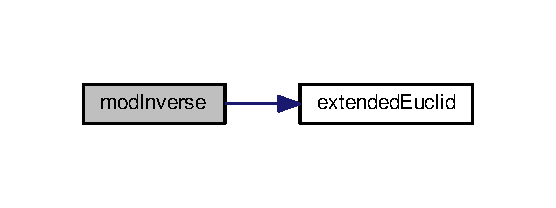
\includegraphics[width=267pt]{EuclidianAlg_8cpp_a95942be30ba56c0c3d82cf4c89fbdcdb_cgraph}
\end{center}
\end{figure}



%--- End generated contents ---

% Index
\backmatter
\newpage
\phantomsection
\clearemptydoublepage
\addcontentsline{toc}{chapter}{Index}
\printindex

\end{document}
